% westcoast cheat sheet: two landscape A4 pages.  Build: make cheatsheet
% Every number here comes from lib/west_ctl.h and lib/west_voice.h
% (dial values printed from that code).
\documentclass{article}
\usepackage[a4paper,landscape,margin=6mm]{geometry}
\usepackage[T1]{fontenc}
\usepackage{lmodern}
\usepackage[default]{sourcesanspro}
\usepackage{amssymb}
\usepackage{amsmath}
\usepackage{tikz}
\usepackage[most]{tcolorbox}
\usepackage{array}
\usepackage{tabularx}
\pagestyle{empty}
\setlength{\parindent}{0pt}

\definecolor{ink}{RGB}{30,30,30}
\definecolor{oscc}{RGB}{170,90,20}     % complex oscillator
\definecolor{foldc}{RGB}{190,40,60}    % folder
\definecolor{funcc}{RGB}{150,60,170}   % function generator
\definecolor{lpgc}{RGB}{30,90,170}     % low-pass gate
\definecolor{rndc}{RGB}{0,130,120}     % uncertainty
\definecolor{freec}{RGB}{170,170,170}  % unassigned
\definecolor{padc}{RGB}{120,170,230}

\newcommand{\OS}[1]{\textcolor{oscc}{#1}}
\newcommand{\FO}[1]{\textcolor{foldc}{#1}}
\newcommand{\FN}[1]{\textcolor{funcc}{#1}}
\newcommand{\LG}[1]{\textcolor{lpgc}{#1}}
\newcommand{\RN}[1]{\textcolor{rndc}{#1}}
\newcommand{\FR}[1]{\textcolor{freec}{#1}}
\newcommand{\cc}[1]{\textcolor{black!45}{\fontsize{4.6}{5}\selectfont #1}}

% knob: x, label
\newcommand{\knob}[2]{%
  \draw[fill=black!8, draw=black!60, line width=0.4pt] (#1,63) circle (3.4);
  \draw[black!60, line width=0.5pt] (#1,63) -- ++(110:2.9);
  \node[font=\fontsize{5.4}{6}\selectfont\bfseries, text=ink, align=center] at (#1,70.2) {#2};}
\newcommand{\pad}[3]{%
  \draw[rounded corners=0.8mm, fill=padc!35!white, draw=padc!80!black, line width=0.4pt]
    (36+#1*13.2, 19+#2*13.2) rectangle ++(12,12);
  \node[font=\fontsize{5.4}{6}\selectfont, text=ink, align=center, text width=11mm]
    at (36+#1*13.2+6, 19+#2*13.2+6) {#3};}
\newcommand{\fader}[3]{%
  \draw[fill=black!12, draw=black!50] (#1-0.7,26) rectangle (#1+0.7,50);
  \draw[fill=#3!60!white, draw=#3!70!black, rounded corners=0.4mm] (#1-2.6,36) rectangle (#1+2.6,40);
  \node[font=\fontsize{5.4}{6}\selectfont\bfseries, text=#3!70!black, align=center] at (#1,55) {#2};}
\newcommand{\btn}[5]{%
  \draw[rounded corners=0.6mm, fill=#4!25!white, draw=#4!70!black, line width=0.4pt]
    (#1-#5/2,#2-2.6) rectangle (#1+#5/2,#2+2.6);
  \node[font=\fontsize{4.9}{5.4}\selectfont, text=ink, align=center] at (#1,#2) {#3};}

\tcbset{card/.style={enhanced, colback=white, colframe=black!70, boxrule=0.5pt, arc=1.5mm,
    left=1.6mm, right=1.6mm, top=1.1mm, bottom=1.1mm, toptitle=0.6mm, bottomtitle=0.6mm,
    fonttitle=\bfseries\fontsize{8.6}{10}\selectfont, coltitle=white, colbacktitle=black!75,
    fontupper=\fontsize{7.1}{8.5}\selectfont, before skip=0mm, after skip=1.8mm}}
\newtcolorbox{card}[1]{card, title={#1}}
\newcolumntype{L}{>{\raggedright\arraybackslash}X}

\begin{document}

{\fontsize{16}{18}\selectfont\bfseries westcoast}\hspace{3mm}%
{\fontsize{9.5}{11}\selectfont Axoloti Core + Launchkey 49 MK3 (standalone mode) \textperiodcentered{}
four voices after Buchla's 259, 292, 281, 266 \textperiodcentered{} \texttt{patches/westcoast/westcoast\_v1.axp}}\hfill
{\fontsize{7}{8}\selectfont\color{black!55} v1.0 \textperiodcentered{} 2026-11-25 \textperiodcentered{} page 1 of 2}

\vspace{1.5mm}
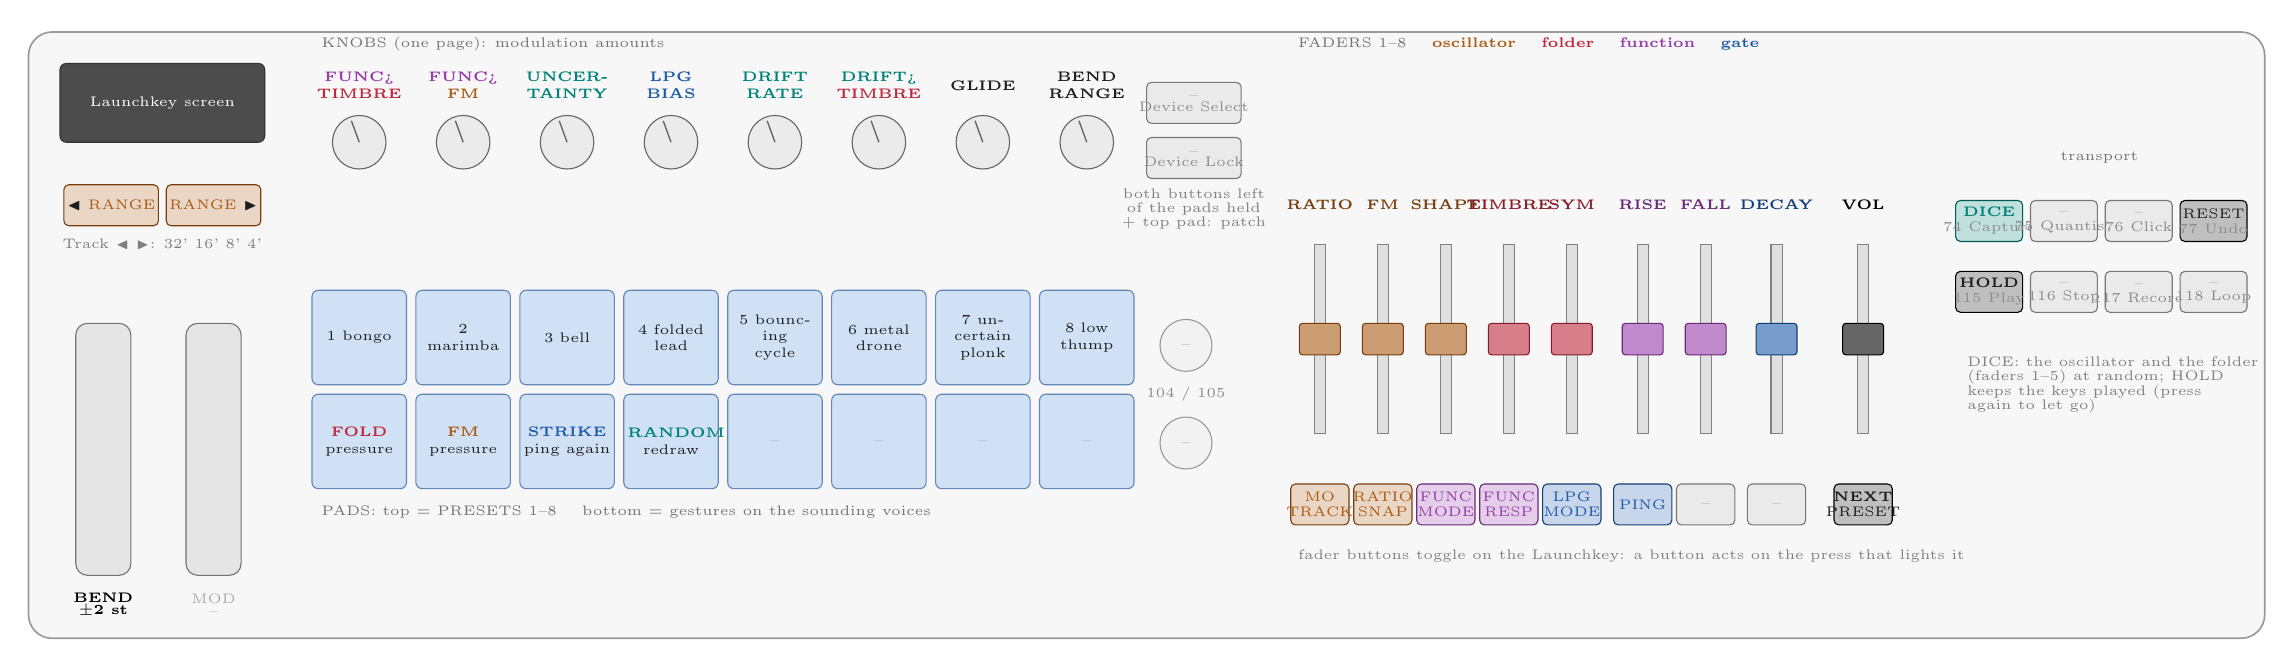
\begin{tikzpicture}[x=1mm,y=1mm]
  \draw[rounded corners=3mm, fill=black!3, draw=black!40, line width=0.6pt] (0,0) rectangle (284,77);

  % ---- left: screen, track buttons, wheels
  \draw[fill=black!70, draw=black!80, rounded corners=0.8mm] (4,63) rectangle (30,73);
  \node[font=\fontsize{5}{6}\selectfont, text=white] at (17,68) {Launchkey screen};
  \btn{10.5}{55}{\(\blacktriangleleft\) \OS{RANGE}}{oscc}{12}
  \btn{23.5}{55}{\OS{RANGE} \(\blacktriangleright\)}{oscc}{12}
  \node[font=\fontsize{4.6}{5}\selectfont, text=black!50] at (17,50) {Track \(\blacktriangleleft\) \(\blacktriangleright\): 32' 16' 8' 4'};
  \draw[rounded corners=1.5mm, fill=black!10, draw=black!55] (6,8) rectangle (13,40);
  \draw[rounded corners=1.5mm, fill=black!10, draw=black!55] (20,8) rectangle (27,40);
  \node[font=\fontsize{5.4}{6}\selectfont\bfseries, align=center] at (9.5,4.2) {BEND\\[-0.6mm]\(\pm\)2 st};
  \node[font=\fontsize{5.4}{6}\selectfont, align=center, text=freec] at (23.5,4.2) {MOD\\[-0.6mm]--};

  % ---- knobs: one page
  \node[font=\fontsize{5}{6}\selectfont, text=black!55, anchor=west] at (36,75.5) {KNOBS (one page): modulation amounts};
  \knob{42}{\FN{FUNC>}\\\FO{TIMBRE}}
  \knob{55.2}{\FN{FUNC>}\\\OS{FM}}
  \knob{68.4}{\RN{UNCER-}\\\RN{TAINTY}}
  \knob{81.6}{\LG{LPG}\\\LG{BIAS}}
  \knob{94.8}{\RN{DRIFT}\\\RN{RATE}}
  \knob{108}{\RN{DRIFT>}\\\FO{TIMBRE}}
  \knob{121.2}{GLIDE}
  \knob{134.4}{BEND\\RANGE}
  \btn{148}{68}{\FR{--}\\[-0.4mm]\cc{Device Select}}{freec}{12}
  \btn{148}{61}{\FR{--}\\[-0.4mm]\cc{Device Lock}}{freec}{12}
  \node[font=\fontsize{4.4}{5}\selectfont, text=black!50, align=center] at (148,54.5) {both buttons left\\of the pads held\\+ top pad: patch};

  % ---- pads
  \pad{0}{1}{1 bongo} \pad{1}{1}{2 marimba} \pad{2}{1}{3 bell} \pad{3}{1}{4 folded\\lead}
  \pad{4}{1}{5 bouncing\\cycle} \pad{5}{1}{6 metal\\drone} \pad{6}{1}{7 uncertain\\plonk} \pad{7}{1}{8 low\\thump}
  \pad{0}{0}{\FO{\textbf{FOLD}}\\pressure} \pad{1}{0}{\OS{\textbf{FM}}\\pressure} \pad{2}{0}{\LG{\textbf{STRIKE}}\\ping again} \pad{3}{0}{\RN{\textbf{RANDOM}}\\redraw}
  \pad{4}{0}{\FR{--}} \pad{5}{0}{\FR{--}} \pad{6}{0}{\FR{--}} \pad{7}{0}{\FR{--}}
  \node[font=\fontsize{5}{6}\selectfont, text=black!55, anchor=west] at (36,16) {PADS: top = PRESETS 1--8 \quad bottom = gestures on the sounding voices};
  \draw[fill=black!5, draw=black!40] (147,37.2) circle (3.3);
  \draw[fill=black!5, draw=black!40] (147,24.8) circle (3.3);
  \node[font=\fontsize{4.6}{5}\selectfont, text=freec] at (147,37.2) {--};
  \node[font=\fontsize{4.6}{5}\selectfont, text=freec] at (147,24.8) {--};
  \node[font=\fontsize{4.2}{5}\selectfont, text=black!45] at (147,31) {104 / 105};

  % ---- faders: the timbre is played here
  \node[font=\fontsize{5}{6}\selectfont, text=black!55, anchor=west] at (160,75.5) {FADERS 1--8 \quad
     \OS{\textbf{oscillator}} \quad \FO{\textbf{folder}} \quad \FN{\textbf{function}} \quad \LG{\textbf{gate}}};
  \fader{164}{RATIO}{oscc} \fader{172}{FM}{oscc} \fader{180}{SHAPE}{oscc}
  \fader{188}{TIMBRE}{foldc} \fader{196}{SYM}{foldc}
  \fader{205}{RISE}{funcc} \fader{213}{FALL}{funcc}
  \fader{222}{DECAY}{lpgc}
  \fader{233}{VOL}{black}
  \btn{164}{17}{\OS{MO}\\\OS{TRACK}}{oscc}{7.4}
  \btn{172}{17}{\OS{RATIO}\\\OS{SNAP}}{oscc}{7.4}
  \btn{180}{17}{\FN{FUNC}\\\FN{MODE}}{funcc}{7.4}
  \btn{188}{17}{\FN{FUNC}\\\FN{RESP}}{funcc}{7.4}
  \btn{196}{17}{\LG{LPG}\\\LG{MODE}}{lpgc}{7.4}
  \btn{205}{17}{\LG{PING}}{lpgc}{7.4}
  \btn{213}{17}{\FR{--}}{freec}{7.4}
  \btn{222}{17}{\FR{--}}{freec}{7.4}
  \btn{233}{17}{\textbf{NEXT}\\PRESET}{black}{7.4}
  \node[font=\fontsize{4.6}{5}\selectfont, text=black!50, anchor=west] at (160,10.5) {fader buttons toggle on the Launchkey: a button acts on the press that lights it};

  % ---- transport (ch 16)
  \node[font=\fontsize{5}{6}\selectfont, text=black!55] at (263,61) {transport};
  \btn{249}{53}{\RN{\textbf{DICE}}\\\cc{74 Capture}}{rndc}{8.5}
  \btn{258.5}{53}{\FR{--}\\\cc{75 Quantise}}{freec}{8.5}
  \btn{268}{53}{\FR{--}\\\cc{76 Click}}{freec}{8.5}
  \btn{277.5}{53}{RESET\\\cc{77 Undo}}{black}{8.5}
  \btn{249}{44}{\textbf{HOLD}\\\cc{115 Play}}{black}{8.5}
  \btn{258.5}{44}{\FR{--}\\\cc{116 Stop}}{freec}{8.5}
  \btn{268}{44}{\FR{--}\\\cc{117 Record}}{freec}{8.5}
  \btn{277.5}{44}{\FR{--}\\\cc{118 Loop}}{freec}{8.5}
  \node[font=\fontsize{4.6}{5.2}\selectfont, text=black!50, align=left, anchor=north west] at (245,37)
     {DICE: the oscillator and the folder\\(faders 1--5) at random; HOLD\\keeps the keys played (press\\again to let go)};
\end{tikzpicture}

\vspace{1.2mm}
\begin{minipage}[t]{72mm}\vspace{0pt}
\begin{card}{Signal path (per voice, four voices)}
\OS{MODULATION OSC} (sine \(\to\) triangle \(\to\) square) \(\to\) through-zero \OS{FM} of the
\OS{PRINCIPAL} sine \(\to\) \FO{FOLDER} (TIMBRE, SYMMETRY) \(\to\) \LG{LOW-PASS GATE} \(\to\) out
(mono). The \FN{FUNCTION} moves the fold, the FM and, without PING, the gate. \RN{UNCERTAINTY}:
a random value per note, and a slow random drift on the fold.
\end{card}
\begin{card}{Complex oscillator}
\OS{\textbf{RATIO}}: the modulator's frequency, 0.25 to 8 times the note's; \OS{RATIO SNAP} pulls it to
1/4, 1/3, 1/2, 2/3, 1, 3/2, 2, 5/2, 3, 4, 5, 6, 7, 8 (harmonic); off, any ratio (bells, gongs).
\OS{MO TRACK} off: the modulator runs free and RATIO is its rate (0.05--820 Hz).
\OS{\textbf{FM}} index 0--8: above 1 the principal runs backwards for part of each cycle
(through zero).
\end{card}
\end{minipage}\hfill
\begin{minipage}[t]{70mm}\vspace{0pt}
\begin{card}{Folder (faders 4, 5)}
\FO{\textbf{TIMBRE}} 0: the plain sine, rounding off up to 1/8; the first fold at 1/4, up to four each way at the top.
The harmonics follow Bessel functions, as on a 259's timbre section. \FO{\textbf{SYMMETRY}} off
centre adds the even harmonics (a hollow sound becomes a buzzy one).
\end{card}
\begin{card}{Low-pass gate (fader 8, buttons 5, 6)}
A \LG{vactrol}: it opens in 1.5 ms and closes with a long tail (\LG{DECAY}). \LG{\textbf{PING}}: each key
strikes it, as hard as the key (the bongo); off: it follows the \FN{function}. \LG{LPG MODE}: COMBO
closes the tone and the level together, LP the tone only, VCA the level only. \LG{LPG BIAS}
holds it partly open.
\end{card}
\end{minipage}\hfill
\begin{minipage}[t]{66mm}\vspace{0pt}
\begin{card}{Function generator (faders 6, 7, buttons 3, 4)}
\FN{\textbf{RISE}}, \FN{\textbf{FALL}}: 0.5 ms--10 s. \FN{FUNC MODE}: TRANSIENT (rises and falls on
each key), SUSTAIN (holds while the key is down), CYCLE (loops while the key is down: an LFO
that starts with the note). \FN{FUNC RESP}: log, lin, exp. FUNC>TIMBRE and FUNC>FM set how
much it folds and modulates.
\end{card}
\begin{card}{Uncertainty, pads, dice}
\RN{UNCERTAINTY}: each note draws its own fold (\(\pm\)0.4) and FM (\(\pm\)2) offsets; \RN{RANDOM}
(bottom pad 4) redraws them for the sounding notes. \RN{DRIFT}: a smooth random on the fold.
FOLD, FM pads: velocity, then pressure, add up to a full fold or +4 FM. \LG{STRIKE}: pings the
sounding voices again.
\end{card}
\end{minipage}\hfill
\begin{minipage}[t]{68mm}\vspace{0pt}
\begin{card}{Inside}
\fontsize{6.6}{7.8}\selectfont
The voices run at 96 kHz and are summed before one half-band filter (\(-79\) dB) to 48 kHz.
Sines from a 1024-point table (error \(< 10^{-5}\)). The folder's harmonics match the
Jacobi--Anger expansion \(2 J_n(\beta)\) (to \(7\cdot10^{-6}\)), the FM sidebands \(J_k(I/r)\)
(to 0.8\,\%); aliasing at full fold \(-83\) dB. Vactrol: \(\dot d = -(6d^2 + d)/T\).
Code: \texttt{lib/west\_voice.h}.
\end{card}
\begin{card}{Load}
DSP 13\,\% idle, 74.5\,\% with four voices held and the gate open; patch RAM 15 of 44 KB.
\end{card}
\end{minipage}

%======================================================================
\newpage
{\fontsize{16}{18}\selectfont\bfseries westcoast}\hspace{3mm}%
{\fontsize{9.5}{11}\selectfont presets, dial values, recipes, troubleshooting}\hfill
{\fontsize{7}{8}\selectfont\color{black!55} v1.0 \textperiodcentered{} page 2 of 2}

\vspace{1.5mm}
\begin{minipage}[t]{150mm}\vspace{0pt}
\begin{card}{Presets: top pads = 1--8; NEXT PRESET (fader button 9) steps; RESET (Undo) = 1 \quad\textmd{\fontsize{6.5}{7}\selectfont (set from the parameter meanings, not yet tuned by ear)}}
\fontsize{7.2}{8.7}\selectfont
\begin{tabularx}{\linewidth}{@{}>{\bfseries}l L@{}}
1 bongo & Ratio 1, a little FM (0.3) and fold; each key pings the gate (COMBO), which closes in about 0.2 s. The power-on sound. \\
2 marimba & The modulator at 4 times the pitch, FM 1 (more as the function falls), a pinged gate with a 0.34 s tail. \\
3 bell & An inharmonic ratio (3.63, no snap), FM 2.4, the plain sine core, a VCA gate with a 1.3 s tail, at 4'. \\
4 folded lead & SUSTAIN function (17 ms up, 0.38 s down) opens the gate and adds fold; fold 0.47, symmetry off centre, drift, glide 0.15 s. \\
5 bouncing cycle & The function CYCLEs (3.5 ms up, 54 ms down) while the key is held: the gate, fold and FM bounce; ratio 2. \\
6 metal drone & The modulator runs free at 4.9 Hz with FM 4 (through zero), fold 0.6, symmetry 0.4, LP gate, 16', drifting. \\
7 uncertain plonk & Uncertainty 0.87: every strike differs in fold and FM; ratio 1.43; a faster drift. \\
8 low thump & 16', the modulator at half the pitch, FM 1.5, fold 0.28, a pinged gate with a 0.47 s tail. \\
\end{tabularx}\\[0.3mm]
A preset sets the switches, faders 1--8 and the knobs; the volume stays. After a preset a fader or knob moves its
value from where it is (no jump); it catches up at the end of its travel at the latest.
\end{card}

\begin{card}{Recipes}
\fontsize{7.4}{9.0}\selectfont
\textbf{Plonk}: PING, COMBO, DECAY at 1/3, FM at 1/4, TIMBRE low; play softly and hard.\quad
\textbf{Bell}: RATIO SNAP off, RATIO between 3/4 and 4/5 of its travel, FM at 1/2, LPG VCA, DECAY at 3/4.\quad
\textbf{Folded lead}: PING off, FUNC SUSTAIN, TIMBRE at 1/2, FUNC>TIMBRE at 1/3, SYMMETRY off centre.\quad
\textbf{Bounce}: FUNC CYCLE, RISE short, FALL at 1/3: the gate bounces while the key is held.\quad
\textbf{Drone}: MO TRACK off (RATIO = a slow rate), LPG BIAS up, HOLD.\quad
\textbf{Chance}: UNCERTAINTY at 3/4, then the STRIKE and RANDOM pads.
\end{card}
\end{minipage}\hfill
\begin{minipage}[t]{128mm}\vspace{0pt}
\begin{card}{Where the values fall (fader or knob at \dots)}
\fontsize{7.3}{8.9}\selectfont
\setlength{\tabcolsep}{3pt}
\begin{tabular}{@{}l r r r r r@{}}
 & 0 & 1/4 & 1/2 & 3/4 & full \\ \hline
\OS{\textbf{RATIO}} (\(\times\) the note) & 0.25 & 0.6 & 1.43 & 3.34 & 8 \\
\OS{\textbf{RATIO}}, SNAP on & 1/4 & 2/3 & 3/2 & 3 & 8 \\
\OS{\textbf{RATIO}}, MO TRACK off (Hz) & 0.05 & 0.58 & 6.6 & 71 & 820 \\
\OS{\textbf{FM}} (index) & 0 & 0.5 & 2 & 4.5 & 8 \\
\OS{\textbf{SHAPE}} & sine & & triangle & & square \\
\FO{\textbf{TIMBRE}} (folds each way) & sine & 1 & 2 & 3 & 4 \\
\FO{\textbf{SYMMETRY}} & \(-1\) & \(-0.5\) & 0 & \(+0.5\) & \(+1\) \\
\FN{\textbf{RISE, FALL}} (s) & 0.0005 & 0.006 & 0.074 & 0.82 & 10 \\
\LG{\textbf{DECAY}} (s) & 0.02 & 0.07 & 0.25 & 0.85 & 3 \\
\FN{\textbf{FUNC>FM}} (index) & 0 & 0.25 & 1 & 2.2 & 4 \\
\LG{\textbf{LPG BIAS}} (open) & 0 & 0.06 & 0.25 & 0.56 & 1 \\
\RN{\textbf{DRIFT RATE}} (Hz) & 0.05 & 0.23 & 1 & 4.4 & 20 \\
\textbf{GLIDE} (s) & 0 & 0.13 & 0.51 & 1.1 & 2 \\
\textbf{BEND RANGE} (st) & 0 & 3 & 6 & 9 & 12 \\
\end{tabular}
\end{card}

\begin{card}{Something seems wrong?}
\fontsize{7.3}{8.9}\selectfont
\textbf{Silence}: PING off with the function in TRANSIENT and a short RISE and FALL (the gate barely opens),
LP mode with the gate closed, DECAY short with soft keys, or VOL down.\quad
\textbf{A note that will not stop}: HOLD (Play), LPG BIAS up, or the function on SUSTAIN or CYCLE with the key down.\quad
\textbf{Harsh}: FM high (through zero), TIMBRE high, SHAPE square.\quad
\textbf{Out of tune}: RATIO SNAP off (inharmonic on purpose), MO TRACK off, or a high FM.\quad
\textbf{A button needs two presses}: the fader buttons toggle; they act on the press that lights them.\quad
\textbf{Lost}: RESET (Undo).\quad
\textbf{Another patch} (on the SD card): hold both buttons left of the pads and tap a top pad: 1 freak,
2 grains, 3 groove, 4 soliton, 5 aeolian, 6 raw, 7 quartet, 8 westcoast.
\end{card}
\end{minipage}

\end{document}
